
\begin{figure}
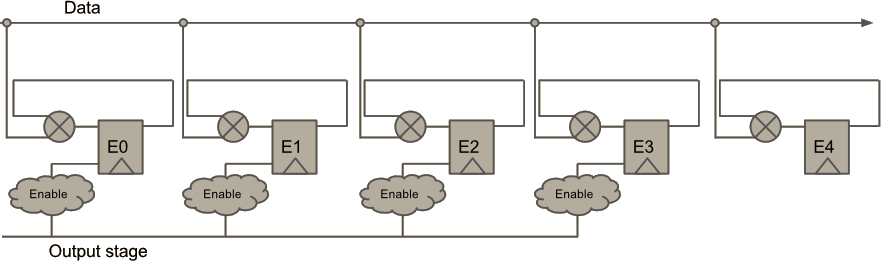
\includegraphics[width=15cm]{implementation/fig_ecc}
\caption{Implementation of Hamming(16,11)}
\label{fig:ecc}
\end{figure}

In this section, we describe how the module designs detailed in
\autoref{sec:design} are implemented on the FPGA. 

\subsection{Technology Schematic}
\label{sec:technologyschematic}

Figure \autoref{fig:technologyschematic} shows how each functionality of
the Liaison from \autoref{fig:overview} is mapped to the LUTs in the syntesised design.
Each functionality are marked with a distinct colour. Note that LUTs marked as either
``Status Calculation'' or ``State Maintenance'' functionality are both a part of the
State Maintenance module.


\begin{figure}[p]
  \vspace*{-1.2in}
  \centerline{ 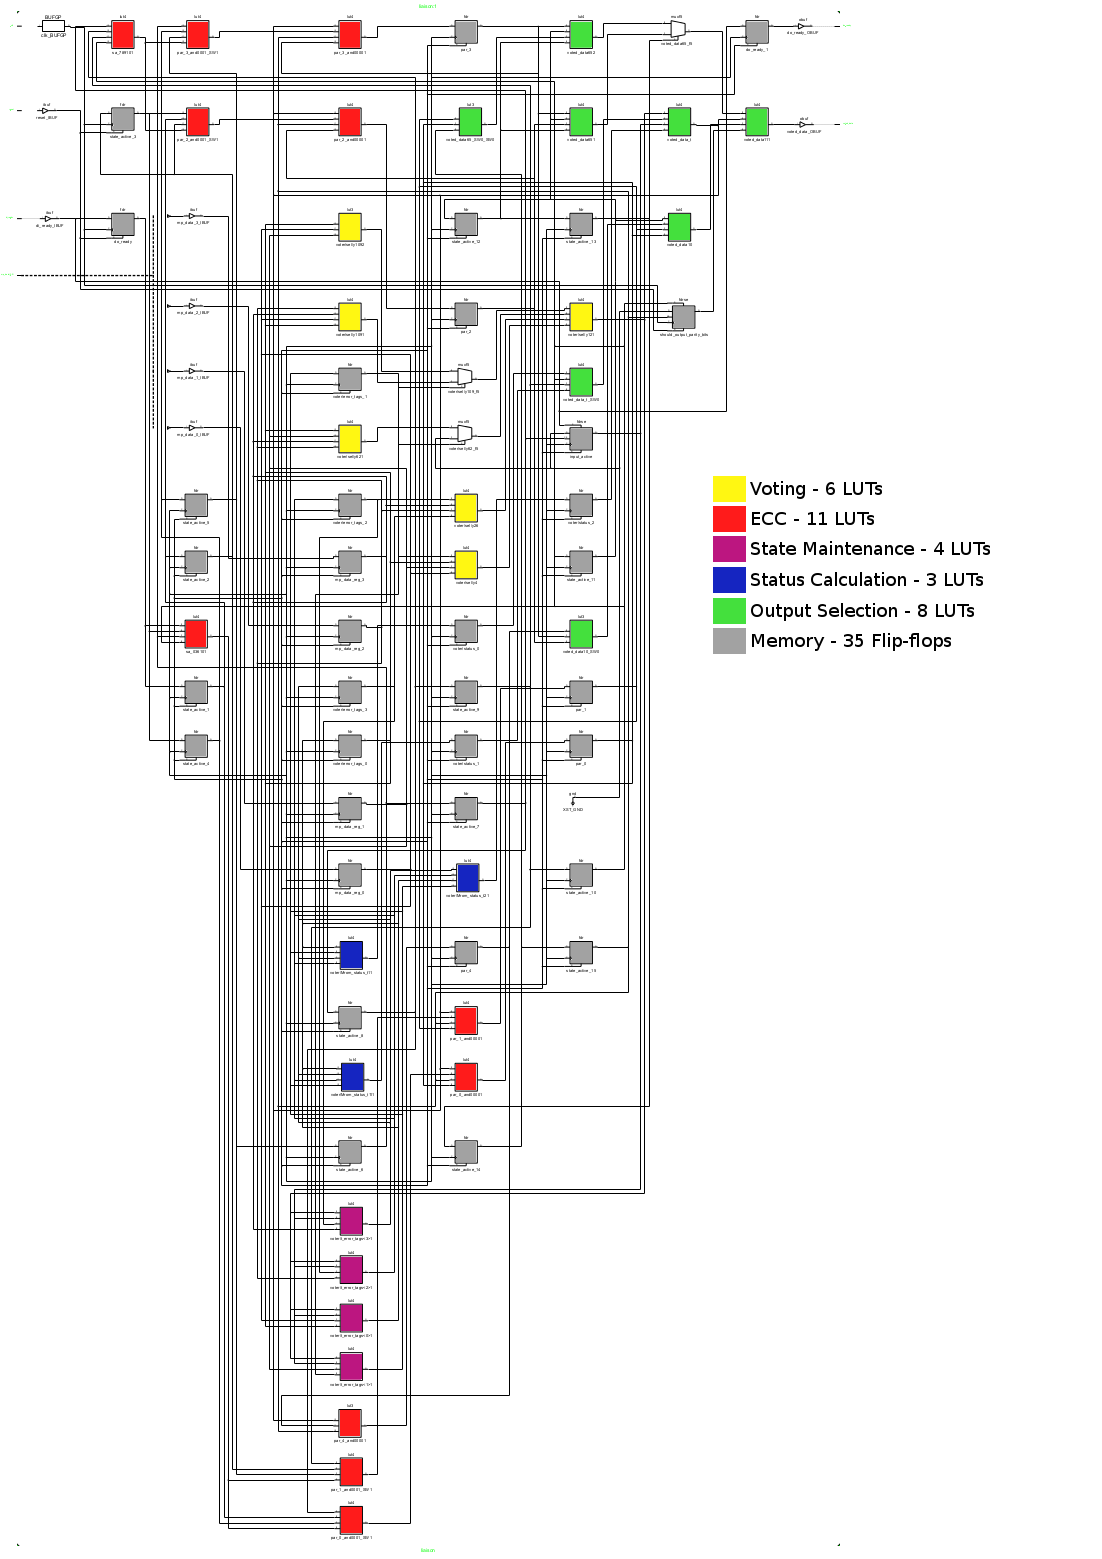
\includegraphics[width=1.2\textwidth]{LUT-count} }
  \caption{The technology schematic of our Liaison}
  \label{fig:technologyschematic}
\end{figure}

\subsection{Voting Algorithm Implementation}
Our design 

\subsection{State Maintenance Implementation}

\subsection{Error Correction Code Implementation}

\subsection{Output Selection Implementation}

\subsection{Results}

\todo[inline]{Describe LUT usage, register usage and clock frequency}
